% -----------------------------------------------------------------
% Section 5.7: Decision Consequences of Missing Metadata
%   Drop-in addition after Section 5.6 (Case Study).
%   Requires: figures/fig8_decision_simulation.pdf
% -----------------------------------------------------------------

\subsection{Decision Consequences of Missing Metadata}\label{sec:decision}

The collision analysis in \S\ref{sec:collisions} establishes that
cross-source score gaps exist; we now show these gaps have concrete
consequences for model selection.

\paragraph{Decision tiers.}
We classify each of the 8~independent collision pairs by the
magnitude of the score gap: \textbf{5~of~8 pairs} (62.5\%) fall
within stochastic noise ($|\Delta| \leq 1$~point), \textbf{2~of~8}
(25\%) show meaningful differences ($1 < |\Delta| \leq 5$), and
\textbf{1~of~8} (12.5\%) shows a major discrepancy
($|\Delta| > 5$)---the 32.3-point GPQA gap.

\paragraph{Metadata conditionality.}
The decision impact splits sharply along metadata availability
(Figure~\ref{fig:decision}). The 5~\emph{metadata-present}
pairs---where both harness and n-shot are documented in both
sources---have a mean $|\Delta|$ of \textbf{0.14} points
(max~0.23), all within noise. The 3~\emph{metadata-absent}
pairs---where harness is unknown in at least one source---have a
mean $|\Delta|$ of \textbf{13.08} points, and 1~of~3 exceeds the
major-discrepancy threshold. In short: when metadata is present,
cross-source scores agree; when metadata is absent, they diverge
by up to 32~points with no way to explain why.

\paragraph{GPQA percentile consequence.}
The most extreme collision demonstrates the practical impact. The
OLv2 score of 16.67 on GPQA places Qwen2.5-72B-Instruct at the
\textbf{93.8th~percentile} of all 4{,}465 models evaluated on that
benchmark; the PWC score of 49.0 would place it \emph{above every
model in the OLv2 distribution} (100th~percentile). A
practitioner consulting one source would conclude this is the best
GPQA model in the ecosystem; consulting the other, they would
conclude it is merely above average---because the evaluation
contexts differ in undocumented ways.

These results demonstrate that the metadata gap is not merely a
documentation inconvenience---it determines whether practitioners
can trust leaderboard-driven model selection.

\begin{figure}[t]
\centering
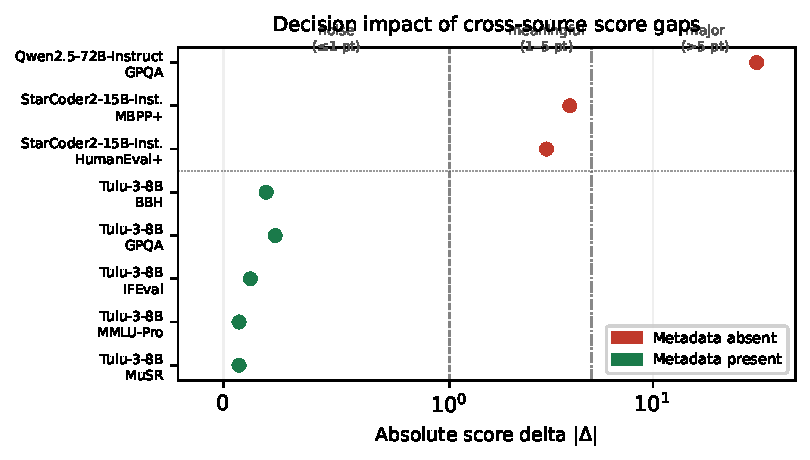
\includegraphics[width=\columnwidth]{figures/fig8_decision_simulation.pdf}
\caption{Decision impact of the 8~independent cross-source collision
pairs. Metadata-present pairs (green; harness and n-shot known in
both sources) cluster within the noise tier ($|\Delta| \leq 1$).
Metadata-absent pairs (red; harness unknown in $\geq$1~source)
scatter across the meaningful and major tiers. Dashed lines mark the
$|\Delta|=1$ and $|\Delta|=5$ decision thresholds.}
\label{fig:decision}
\end{figure}
